\fbox
{
\begin{minipage}{0.45\textwidth}
    \vspace{0.5cm}
    Key findings:
    \begin{itemize}
        \item At large n, the algorithm gives the direction of antineutrino sources
        \item At small n, the algorithm gives a reasonable uncertainty
        \item As a pattern matching method, the algorithm provides a comparison between distributions
    \end{itemize}
\end{minipage}
}
\hspace{0.025\textwidth}
\begin{minipage}{0.45\linewidth}
\begin{figure}
    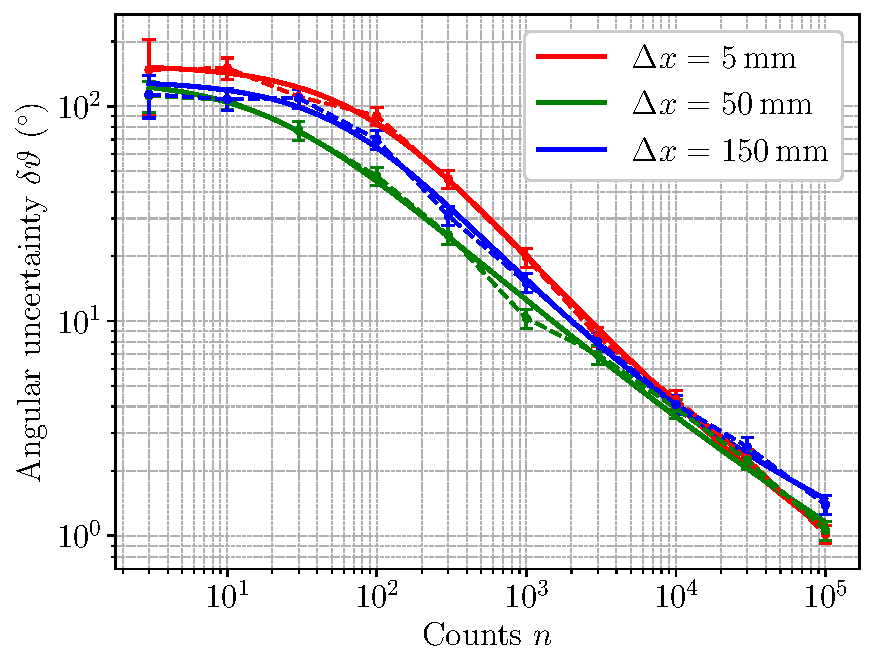
\includegraphics[width=0.7\linewidth]{fig/parallel/06_money_plot_fit_arctan_log_4p.pdf}

    \label{fig:POI_segsize_uncert}
\end{figure}
\end{minipage}
    \captionof{figure}{Angular uncertainty $\delta\vartheta$ versus event count $n$ for square segment sizes of 5, 50, and 150 mm.}
\vspace{0.5cm}

% ---- Figure 6: (a) binning distribution at theta=0  +  (b) sweet-spot plot ----
\begin{figure}
\centering
\begin{tabular}{cc}
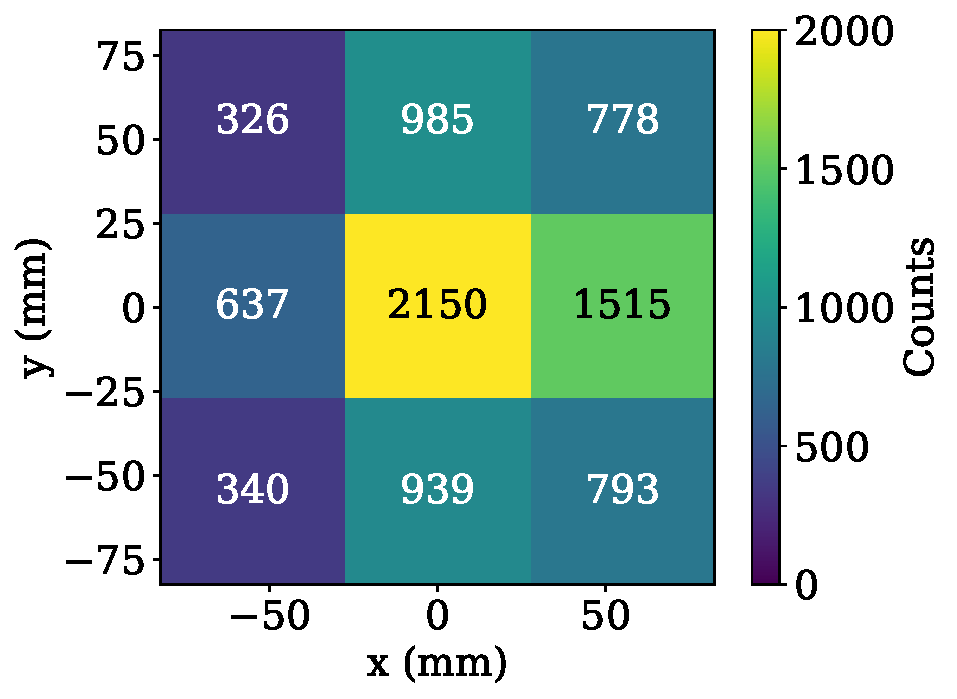
\includegraphics[width=0.32\linewidth]{fig/bin_dist_rot0_001wt.pdf}
&
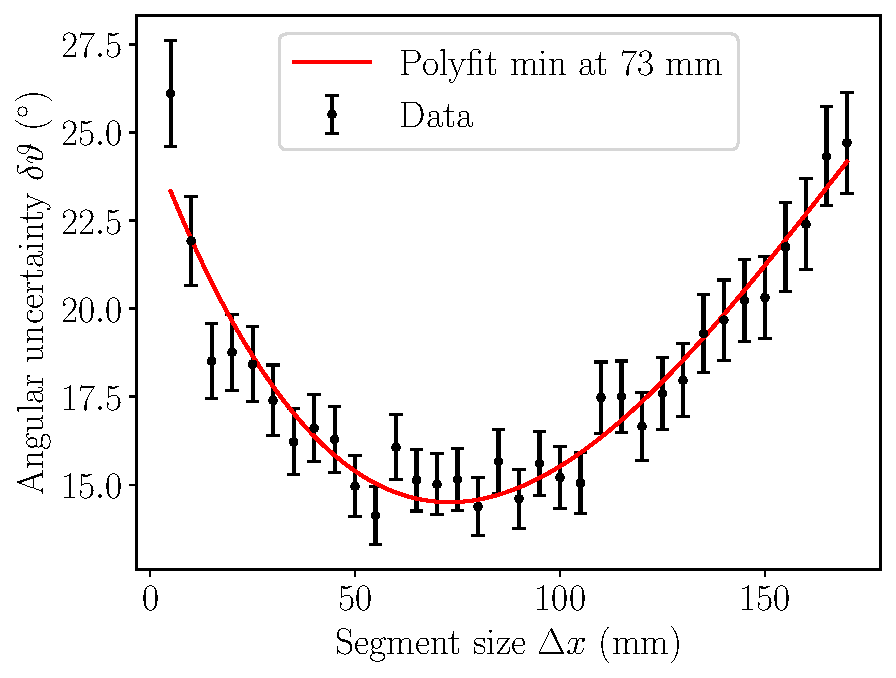
\includegraphics[width=0.45\linewidth]{fig/parallel/sweet_spot_final.pdf} \\
\end{tabular}

\begin{tabular}{>{\centering\arraybackslash}p{0.35\linewidth} >{\centering\arraybackslash}p{0.5\linewidth}}
    \makebox[0.35\linewidth][c]{%
        \begin{picture}(20,20)
            \put(-5,13){\color{black}\vector(1,0){20}}
        \end{picture}
    }
    &
    \\
    (a) binning distribution, $\vartheta_\nu = 0^\circ$ & (b) angular uncertainty vs.\ segment size
\end{tabular}
    \caption{(a) Binning distribution at $\vartheta_\nu=0^\circ$ (0.1\,wt\%\ ${}^6$Li; arrow marks the antineutrino direction); other incoming angles rotate the pattern. (b) Angular uncertainty versus segment size $\Delta x$, with a polynomial fit minimizing near $\Delta x\approx 73$ mm.}
    \label{fig:binning_sweetspot}
\end{figure}

\begin{center}
\highlight{Optimal segment size: $\Delta x \approx 73$ mm}
\end{center}
\vspace{0.3cm}

% ---- Figure 7: FND vs reference angle, labels on the plots (reference style) ----
\begin{figure}
\centering

\begin{minipage}{0.32\textwidth}
    \centering
    \begin{tikzpicture}
        \node[inner sep=0]
            {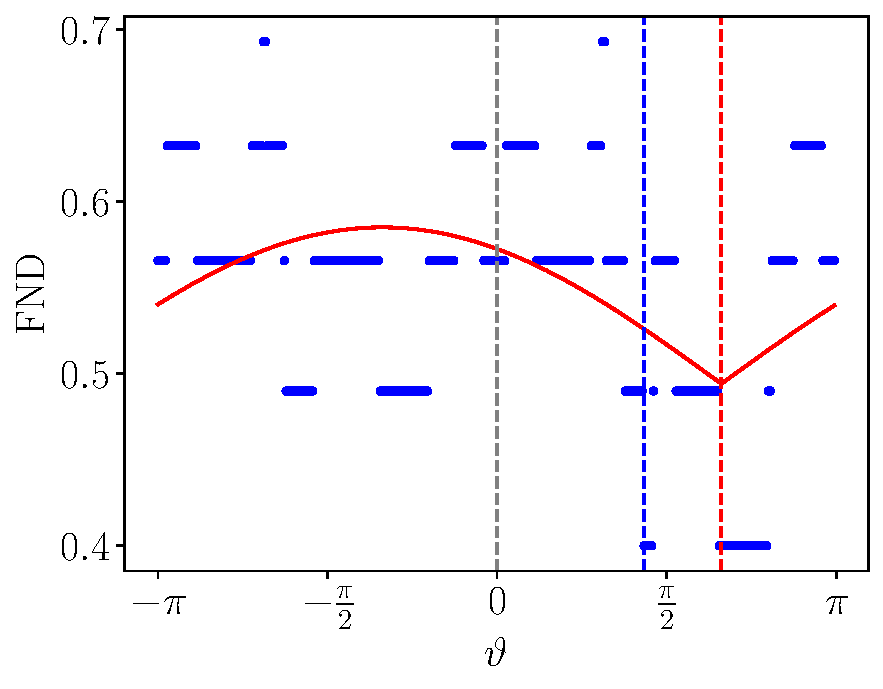
\includegraphics[height=1.675in]{fig/parallel/FND_n_10_dx_50.pdf}};

        \node[red, font=\fontsize{16}{19}\selectfont] at (1.85,2.225) {$\vartheta_\mathrm{fit}$};
        \node[blue, font=\fontsize{16}{19}\selectfont] at (1.15,2.225) {$\vartheta_\mathrm{min}$};
        \node[gray!50!black, font=\fontsize{16}{19}\selectfont] at (0.25,2.225) {$\vartheta_\mathrm{true}$};
    \end{tikzpicture}

    \vspace{2pt}
    (a) $n=10$
\end{minipage}
\hfill
\begin{minipage}{0.32\textwidth}
    \centering
    \begin{tikzpicture}
        \node[inner sep=0]
            {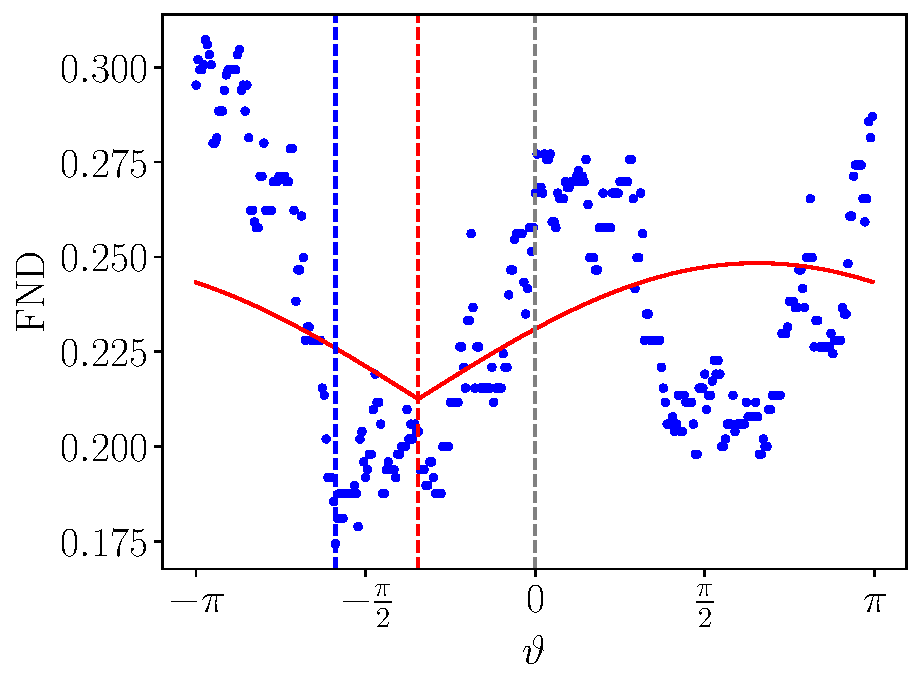
\includegraphics[height=1.675in]{fig/parallel/FND_n_100_dx_50.pdf}};

        \node[red, font=\fontsize{16}{19}\selectfont] at (-0.25,2.23) {$\vartheta_\mathrm{fit}$};
        \node[blue, font=\fontsize{16}{19}\selectfont] at (-0.9,2.23) {$\vartheta_\mathrm{min}$};
        \node[gray!50!black, font=\fontsize{16}{19}\selectfont] at (0.45,2.23) {$\vartheta_\mathrm{true}$};
    \end{tikzpicture}

    \vspace{2pt}
    (b) $n=100$
\end{minipage}
\hfill
\begin{minipage}{0.32\textwidth}
    \centering
    \begin{tikzpicture}
        \node[inner sep=0]
            {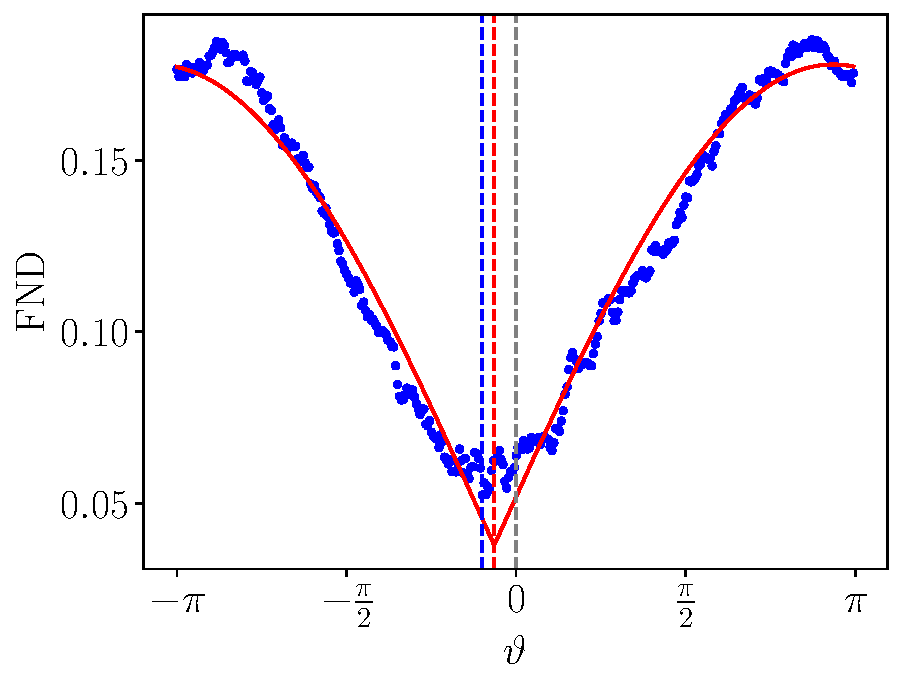
\includegraphics[height=1.675in]{fig/parallel/FND_n_1000_dx_50.pdf}};

        \node[red, font=\fontsize{16}{19}\selectfont] at (0.25,2.23) {$\vartheta_\mathrm{fit}$};
        \node[blue, font=\fontsize{16}{19}\selectfont] at (-0.4,2.23) {$\vartheta_\mathrm{min}$};
        \node[gray!50!black, font=\fontsize{16}{19}\selectfont] at (0.9,2.23) {$\vartheta_\mathrm{true}$};
    \end{tikzpicture}

    \vspace{2pt}
    (c) $n=1000$
\end{minipage}

\caption{FND versus reference angle $\vartheta$ at $n=10,100,1000$ (50 mm segments, RAT-PAC 2 capture data). As $n$ grows, the minimum $\vartheta_\mathrm{min}$ and arctan fit $\vartheta_\mathrm{fit}$ approach the true angle $\vartheta_\mathrm{true}$.}
\label{fig_spread}
\end{figure}


\fbox
{
\begin{minipage}{0.98\textwidth}
\vspace{0.5cm}
    Future work:
        \begin{itemize}
            \item Developing methods to take advantage of machine learning
            \item Investigating how to apply to monolithic detectors
            \item Investigating a generalized approach to three dimensionally segmented detectors
        \end{itemize}
\end{minipage}
}
